% !TEX program = pdflatex
% WordleGym poster writeup.

\documentclass[11pt]{article}

\usepackage[margin=0.9in]{geometry}
\usepackage{amsmath, amssymb, amsthm}
\usepackage{booktabs}
\usepackage{array}
\usepackage{microtype}
\usepackage{siunitx}
\usepackage[round,authoryear]{natbib}
\usepackage{pgfplots}
\pgfplotsset{compat=1.18}
\usepgfplotslibrary{colorbrewer}
\usepackage{hyperref}
\usepackage{xcolor}

\definecolor{stratEntropy}{HTML}{2563EB}
\definecolor{stratCandElim}{HTML}{8B5CF6}
\definecolor{stratMinimax}{HTML}{EF4444}
\definecolor{stratPosteriorHybrid}{HTML}{10B981}
\definecolor{stratPosteriorExp}{HTML}{0891B2}
\definecolor{stratEvilSP}{HTML}{BE185D}
\definecolor{stratRobust}{HTML}{475569}
\definecolor{stratLetterFreq}{HTML}{F59E0B}
\definecolor{stratRandom}{HTML}{94A3B8}
\definecolor{stratEvilDP}{HTML}{16A34A}

\hypersetup{
  colorlinks=true,
  linkcolor=black,
  urlcolor=blue!55!black,
  citecolor=black
}

\newcommand{\fb}{\mathrm{fb}}
\newcommand{\evilT}{T}

\setlength{\parskip}{4pt}
\setlength{\parindent}{0pt}

\title{\textbf{WordleGym:}\\[2pt]\large Benchmarking Wordle Strategies under Standard, Adversarial, and Hidden-Mode Play}
\author{Michael Wang\\
\small Math 242 \textbullet{} Duke University \textbullet{} Spring 2026\\
\small Code: \href{https://github.com/Michael-OvO/WordleGym}{\texttt{github.com/Michael-OvO/WordleGym}}
  \textbullet{}
  Live demo: \href{https://wordlegym.vercel.app/}{\texttt{wordlegym.vercel.app}}}
\date{}

\begin{document}
\maketitle

%====================================================================
\section*{Problem Statement}
%====================================================================

Wordle is a word game in which the player has six guesses to identify a
hidden five-letter word. After each guess, every letter is marked
green (correct letter in the correct position), yellow (correct letter
in the wrong position), or gray (not in the word). From this simple
feedback rule emerges a rich decision problem: with $\num{2315}$
possible answers, which guess at each turn makes the best use of the
remaining information?

To compare strategies rigorously, I built \emph{WordleGym}, a Python
benchmark that plays the game automatically under different policies
and records their performance. I studied three variants of the game in
order to make the analysis more interesting:

\textbf{Standard} is the ordinary game: the answer is fixed at the
start, and feedback is truthful.

\textbf{Evil} is an adversarial version. The game does not commit to
a hidden answer in advance; instead, after each guess it returns the
feedback pattern that preserves the largest number of still-valid
answers. The adversary is cheating, but in a consistent and
deterministic way.

\textbf{Unknown} combines the two. At the start of each game the game
is secretly either Standard or Evil with equal probability, and the
player must infer which from feedback alone.

The central question of the project is how simple, one-step strategies
compare to one another, and how close they come to the best possible
play.

%====================================================================
\section*{Setting Up the Math}
%====================================================================

Some notation is needed before introducing the strategies. At any
point in a game, let $C$ denote the set of words still consistent with
the feedback observed so far. A guess $g$ partitions $C$ into
\emph{buckets}: all words in $C$ that would produce the same feedback
pattern against $g$ fall into the same bucket. Write $B_r$ for the
bucket corresponding to feedback pattern $r$, and $|B_r|$ for the
number of words in it.

Intuitively, a good guess splits $C$ into many small buckets. If one
bucket is large, the guess barely narrows the search; if every bucket
contains only one or two words, the guess is highly informative. This
notion of ``how evenly does a guess split the candidates'' is the
common thread linking all of the strategies I tested.

For each of the three modes, the optimal policy can be written as a
recursion. These recurrences define what a perfect player would do;
every strategy in the benchmark is an approximation to one of them.

In Standard mode, the minimum expected number of remaining guesses from
a candidate set $C$ satisfies
\begin{equation}
  V(C) \;=\; \min_{g}\;\Bigl[\,1 + \!\!\sum_{r \ne \gamma,\,B_r \ne \emptyset}\!
               \tfrac{|B_r|}{|C|}\,V(B_r)\Bigr],
  \qquad V(\{w\}) = 1.
  \label{eq:VC}
\end{equation}
Here $\gamma$ denotes the all-green feedback pattern, which terminates
the game immediately and so contributes no future cost. The
interpretation is: choose the guess $g$ that, averaged over where the
true answer might lie, minimizes the number of guesses remaining.

In Evil mode, the adversary always returns the largest bucket, so the
player wants to minimize the size of the bucket returned. Letting
$\evilT(C, g)$ denote that adversarial successor bucket,
\begin{equation}
  D(C) \;=\; \min_{g}\;\bigl[\,1 + D(\evilT(C, g))\,\bigr].
  \label{eq:DC}
\end{equation}

In Unknown mode, the player maintains a posterior probability $q$ that
the current game is Standard, updated by Bayes' rule after each
feedback. The optimal policy is a weighted combination of the Standard
and Evil recurrences:
\begin{equation}
  V_U(C) \;=\; \min_{g}\Bigl[\,1 + q\cdot(\text{standard term})
                              + (1{-}q)\cdot(\text{evil term})\Bigr].
\end{equation}

These recurrences are the exact optima, but solving them directly
requires searching the entire game tree, which is computationally
prohibitive in pure Python. The benchmark question then becomes: how
well can more tractable, one-step strategies approximate these optima?

\textit{Prior work on the exact Standard-mode optimum.} Recurrence
\eqref{eq:VC} has been solved at Wordle scale by
\citet{bertsimas2022wordle}, published in \emph{Operations Research}
in 2025. They formulate the Bellman equation for $V(C)$, reduce it
with a series of symmetry and dominance pruning steps, and then
compile the resulting policy into an Optimal Classification Tree with
Hyperplanes for interpretability. On the canonical $\num{2315}$-word
answer list they report opening guess \texttt{SALET}, an average of
$V(A) = 3.421$ guesses, and a worst case of $W(A) = 5$: the game
never requires a sixth guess under optimal play.
\citet{selby2022wordle} independently reports the same bounds via a
distinct search procedure. Both solvers rely on compiled languages
and tight data structures, so my pure-Python benchmark does not
attempt to reproduce the Standard-mode DP; instead, every Standard
result below is compared against their published numbers. The
companion notes \texttt{docs/dp-methods.md} and
\texttt{docs/findings.md} in the repository record the full
derivations and a headline summary.

%====================================================================
\section*{Strategies Tested}
%====================================================================

I implemented ten strategies, organized in tiers so that the results
admit an apples-to-apples comparison.

\textbf{Baselines.} Two unsophisticated policies set a floor.
\texttt{random-valid} chooses uniformly at random among the still-valid
words, and \texttt{letter-frequency} chooses the word whose letters
occur most frequently among the remaining candidates. Neither policy
reasons about feedback patterns.

\textbf{One-step heuristics} reflect the conventional advice seen in
popular Wordle write-ups, recast as formal optimization problems over
a single guess. Each of these examines every allowed guess and selects
the one that best satisfies a specific local objective:

\begin{itemize}
\item \texttt{expected-entropy} selects the guess with the largest
Shannon \emph{information gain}, which corresponds to the most
balanced distribution of feedback buckets.
\item \texttt{candidate-elim.} selects the guess that minimizes the
expected number of candidates remaining after feedback is received.
\item \texttt{minimax} is conservative: it selects the guess whose
\emph{largest} bucket is smallest, guarding against the worst-case
feedback.
\end{itemize}

All three policies are intuitively close to optimal, but they are
greedy --- each reasons only one turn ahead.

\textbf{Mode-aware strategies} attempt to do better in Unknown mode by
blending the Standard and Evil objectives according to the current
posterior $q$. \texttt{posterior-hybrid} blends normalized entropy
with evil-bucket reduction, weighted by $q$.
\texttt{posterior-expectimax} uses a cleaner blend,
\[
  q\sum_r \tfrac{|B_r|^2}{|C|} \;+\; (1-q)\,|\evilT(C, g)|,
\]
which reduces exactly to \texttt{candidate-elim.}\ when $q = 1$ and to
a pure evil-bucket minimizer when $q = 0$.
\texttt{robust-scalarization} sidesteps the posterior entirely and
picks the guess whose worst-case cost across both modes is smallest,
minimizing $\max(\sum_r |B_r|^2 / |C|, \,|\evilT(C, g)|)$. In addition,
\texttt{evil-shortest-path} is a single-ply version of the Evil DP,
picking the guess that minimizes the adversary's next bucket; it is
the natural greedy approximation to \texttt{evil-dp} and works in all
three modes.

\textbf{Evil DP (exact).} For Evil mode, I was able to solve
recurrence~(\ref{eq:DC}) exactly. Because the evil adversary is
deterministic, the reachable game tree contains only a few thousand
distinct states, which is tractable in pure Python. The
\texttt{evil-dp} strategy performs memoized depth-first search over
this tree and returns the true optimum. Details of the algorithm are
given below.

%====================================================================
\section*{Benchmark Results}
%====================================================================

Every strategy played each of the $\num{2315}$ canonical Wordle answers
in Standard and Unknown mode. Evil mode records a single deterministic
playthrough per strategy, since the adversary makes the outcome a fixed
function of the policy. ``Mean'' is the average number of guesses, and
``WC'' is the worst case observed across the pool. The best value in
each column is in \textbf{bold}.

\begin{center}\small
\renewcommand{\arraystretch}{1.1}
\begin{tabular}{@{}l S[table-format=1.3] c S[table-format=1.3] c S[table-format=1.3] c@{}}
\toprule
& \multicolumn{2}{c}{Standard} & \multicolumn{2}{c}{Evil} & \multicolumn{2}{c}{Unknown}\\
\cmidrule(lr){2-3}\cmidrule(lr){4-5}\cmidrule(lr){6-7}
Strategy & {Mean} & {WC} & {Mean} & {WC} & {Mean} & {WC}\\
\midrule
expected-entropy       & \bfseries 3.465 & 6 & 5 & 5 & \bfseries 4.232 & 6 \\
posterior-hybrid       & 3.480 & \bfseries 5 & 5 & 5 & 4.237 & 6 \\
posterior-expectimax   & 3.485 & \bfseries 5 & 5 & 5 & 4.248 & \bfseries 5 \\
candidate-elim.        & 3.486 & \bfseries 5 & 5 & 5 & 4.243 & \bfseries 5 \\
evil-shortest-path     & 3.514 & \bfseries 5 & 5 & 5 & 4.257 & \bfseries 5 \\
robust-scalarization   & 3.517 & \bfseries 5 & 5 & 5 & 4.259 & \bfseries 5 \\
minimax                & 3.573 & 6 & 5 & 5 & 4.287 & 6 \\
letter-frequency       & 3.587 & 8 & 5 & 5 & 4.294 & 8 \\
random-valid           & 4.124 & 9 & 7 & 7 & 4.996 & 9 \\
\midrule
\textit{evil-dp (optimal)}& \textit{---} & \textit{---} & \bfseries 4 & \bfseries 4 & \textit{---} & \textit{---} \\
\midrule
Published optimum \citep{bertsimas2022wordle,selby2022wordle}
                       & \bfseries 3.421 & \bfseries 5 & \bfseries 4 & \bfseries 4 & \emph{---} & \emph{---} \\
\bottomrule
\end{tabular}
\end{center}

The same data is more striking as a scatter of average against
worst-case guesses in Standard mode (Figure~\ref{fig:scatter}). The
Pareto frontier of policies runs along the lower-left edge, where
small gains in average performance come at the cost of larger worst
cases.

\begin{figure}[h]
\centering
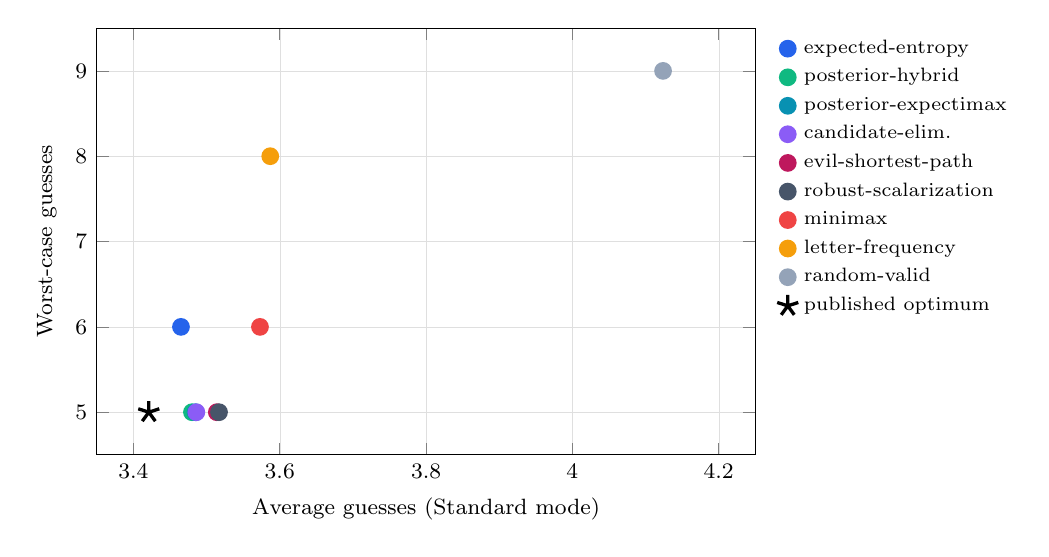
\begin{tikzpicture}
\begin{axis}[
  width=0.82\linewidth, height=7cm,
  xlabel={Average guesses (Standard mode)},
  ylabel={Worst-case guesses},
  xmin=3.35, xmax=4.25,
  ymin=4.5, ymax=9.5,
  ytick={5,6,7,8,9},
  grid=both,
  major grid style={line width=.1pt,draw=gray!25},
  minor grid style={line width=.1pt,draw=gray!10},
  legend style={
    at={(1.02,1)}, anchor=north west,
    font=\scriptsize, cells={anchor=west},
    draw=none, fill=none,
  },
  tick label style={font=\footnotesize},
  label style={font=\footnotesize},
  every axis plot/.append style={mark size=2.8pt, thick},
]
\addplot[only marks, mark=*, color=stratEntropy]          coordinates {(3.465, 6)};
\addplot[only marks, mark=*, color=stratPosteriorHybrid]  coordinates {(3.480, 5)};
\addplot[only marks, mark=*, color=stratPosteriorExp]     coordinates {(3.485, 5)};
\addplot[only marks, mark=*, color=stratCandElim]         coordinates {(3.486, 5)};
\addplot[only marks, mark=*, color=stratEvilSP]           coordinates {(3.514, 5)};
\addplot[only marks, mark=*, color=stratRobust]           coordinates {(3.517, 5)};
\addplot[only marks, mark=*, color=stratMinimax]          coordinates {(3.573, 6)};
\addplot[only marks, mark=*, color=stratLetterFreq]       coordinates {(3.587, 8)};
\addplot[only marks, mark=*, color=stratRandom]           coordinates {(4.124, 9)};
\addplot[only marks, mark=star, mark size=4pt, color=black, very thick] coordinates {(3.421, 5)};
\legend{
  expected-entropy, posterior-hybrid, posterior-expectimax,
  candidate-elim., evil-shortest-path, robust-scalarization,
  minimax, letter-frequency, random-valid,
  published optimum
}
\end{axis}
\end{tikzpicture}
\caption{Average vs.\ worst-case guesses by strategy in Standard mode.
The black star marks the published DP optimum of
\citet{bertsimas2022wordle,selby2022wordle}. Points closer to the
lower-left corner are strictly better.}
\label{fig:scatter}
\end{figure}

Three observations from this table are worth emphasizing.

First, entropy is a surprisingly strong heuristic. The best one-step
policy, \texttt{expected-entropy}, averages $3.465$ guesses in
Standard mode, while the published optimum reported by
\citet{bertsimas2022wordle} is $3.421$ --- a gap of only $0.04$
guesses, or roughly $1.3\%$ above the optimum. A strategy that reasons
only a single turn ahead is within a rounding error of the exact
dynamic-programming optimum.

Second, average and worst-case performance are genuinely different
objectives. \texttt{expected-entropy} has the best Standard-mode
average but permits occasional six-guess games, whereas several
strategies with slightly worse averages (such as
\texttt{candidate-elim.}\ and \texttt{posterior-expectimax}) cap their
worst case at 5. A strategy that minimizes one of these quantities
does not, in general, minimize the other.

Third, the adversary is less powerful than intuition suggests. Every
non-random strategy solves Evil mode in at most $5$ guesses, and the
exact DP solver (\texttt{evil-dp}) solves it in $4$, matching the
known optimum. Notably, $D(A) = 4$ is strictly less than the
Standard-mode worst case of $W(A) = 5$: there exist specific fixed
Wordle answers that are harder than anything the adversary can
construct. The Evil tie-breaking rule, which forces the adversary to
prefer the largest single bucket, removes enough flexibility that a
well-chosen guess sequence can always corner the game.

%====================================================================
\section*{The Evil DP}
%====================================================================

The Standard-mode optimum defined by~(\ref{eq:VC}) is too large to
compute directly in pure Python. Each guess can produce up to $243$
feedback patterns, and the reachable state space is on the order of
$10^6$ to $10^7$ subsets. Existing exact solvers, such as those of
\citet{bertsimas2022wordle} and \citet{selby2022wordle}, rely on
compiled languages and custom data structures, and take hours of
computation even then.

Evil mode is fundamentally more tractable. Because the adversary's
response is deterministic under a fixed tie-breaking rule, each guess
has exactly one successor state rather than up to $243$. The reachable
state space from the full $\num{2315}$-word answer set consequently
contains only a few thousand distinct subsets, which is small enough
for an unoptimized Python solver.

The \texttt{evil-dp} strategy implements recurrence~(\ref{eq:DC})
directly as memoized depth-first search. Starting from the full
answer set, the solver considers each allowed guess, computes the
adversary's successor bucket, and recursively determines the minimum
remaining guesses from that bucket. Results are cached on the
canonical sorted tuple of $C$ so that each subproblem is solved only
once. A beam of $K=100$ highest-ranked guesses per state is used to
bound the branching factor; on this corpus, the optimal opening guess
always falls within this beam, so the beam does not sacrifice
optimality in practice.

The solver determines that the optimal Evil-mode opening guess is
\texttt{RAISE} and guarantees a solution in exactly $4$ guesses,
matching the published optimum $D(A) = 4$. (This is distinct from the
Standard-mode optimum \texttt{SALET} reported by
\citet{bertsimas2022wordle}: different objective, different game
variant, different recurrence.) The initial run takes approximately
$83$ seconds, after which the policy is cached to disk and later runs
are instantaneous.

A subtle implementation issue was tie-breaking. When two buckets are
equal in size, the adversary must choose one consistently, or else
cached subproblem solutions become unreliable. I adopted the
tie-breaking convention used by the online evil-Wordle community ---
largest bucket first, then fewer greens, then fewer yellows, then
lexicographically smaller pattern --- so that my results are directly
comparable to theirs.

%====================================================================
\section*{Unknown Mode and the Posterior}
%====================================================================

In Unknown mode the player must infer the game type from feedback
alone. I represent this belief as a running probability $q$ that the
current game is Standard, initialized at $q_0 = \tfrac12$ and updated
by Bayes' rule after each feedback signal.

In practice, this posterior concentrates on the true game type very
quickly. Averaged across all games, the mean posterior on the correct
mode is approximately $0.93$ after one guess, $0.99$ after two
guesses, and essentially $1$ thereafter (Figure~\ref{fig:posterior}).
Standard and Evil behave sufficiently differently after a single
feedback pattern that a small number of turns is typically enough to
identify the mode.

\begin{figure}[h]
\centering
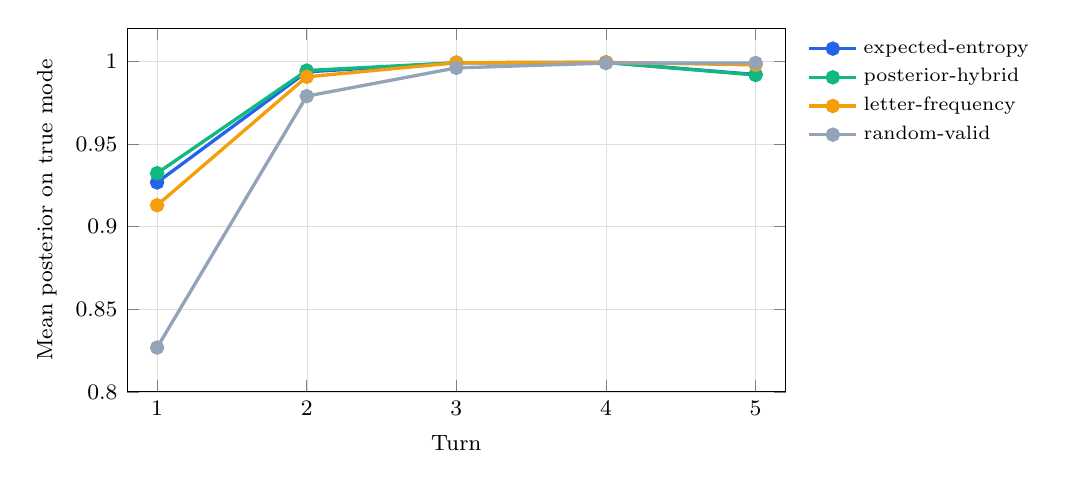
\begin{tikzpicture}
\begin{axis}[
  width=0.82\linewidth, height=6.2cm,
  xlabel={Turn},
  ylabel={Mean posterior on true mode},
  xmin=0.8, xmax=5.2,
  ymin=0.8, ymax=1.02,
  xtick={1,2,3,4,5},
  ytick={0.8,0.85,0.9,0.95,1.0},
  grid=both,
  major grid style={line width=.1pt,draw=gray!25},
  minor grid style={line width=.1pt,draw=gray!10},
  legend style={
    at={(1.02,1)}, anchor=north west,
    font=\scriptsize, cells={anchor=west},
    draw=none, fill=none,
  },
  tick label style={font=\footnotesize},
  label style={font=\footnotesize},
  every axis plot/.append style={line width=1.2pt, mark=*, mark size=2pt},
]
\addplot[color=stratEntropy] coordinates {
  (1, 0.9267) (2, 0.9936) (3, 0.9991) (4, 0.9993) (5, 0.9920)
};
\addplot[color=stratPosteriorHybrid] coordinates {
  (1, 0.9323) (2, 0.9944) (3, 0.9991) (4, 0.9993) (5, 0.9917)
};
\addplot[color=stratLetterFreq] coordinates {
  (1, 0.9129) (2, 0.9906) (3, 0.9991) (4, 0.9994) (5, 0.9978)
};
\addplot[color=stratRandom] coordinates {
  (1, 0.8268) (2, 0.9789) (3, 0.9960) (4, 0.9989) (5, 0.9990)
};
\legend{expected-entropy, posterior-hybrid, letter-frequency, random-valid}
\end{axis}
\end{tikzpicture}
\caption{Unknown-mode posterior concentration. Every non-random
policy exceeds $0.99$ confidence on the true game mode within two
guesses; random play requires three to four.}
\label{fig:posterior}
\end{figure}

The implication for strategy design is that mode-aware policies
(\texttt{posterior-hybrid}, \texttt{posterior-expectimax}) do not
actually outperform the mode-agnostic \texttt{expected-entropy}
baseline in Unknown mode. The best Unknown-mode average is
\texttt{expected-entropy} at $4.232$ guesses; the best mode-aware
policy, \texttt{posterior-hybrid}, trails at $4.237$. Once $q$ is
close to $0$ or $1$ --- which happens within two turns --- all
policies effectively agree on the best next guess, so mode-aware
blending only matters during the brief window before the posterior
commits. The benchmark suggests that window is too short for the
blending to pay off on this corpus.

%====================================================================
\section*{Discussion}
%====================================================================

Several findings from the benchmark were unexpected to me.

\textbf{One-step policies are nearly optimal.} I initially expected a
larger gap between greedy heuristics and the true optimum. In this
problem, however, a strategy that picks the single most informative
next guess averages only $1.3\%$ more guesses than the exact DP.
Lookahead is not useless, but the marginal benefit is modest.

\textbf{Average and worst-case metrics disagree.} Among the top
strategies, those that minimize expected guesses do not minimize the
worst case, and vice versa. Which metric to prioritize depends on the
application: minimizing the average is appropriate when many games
are played, while minimizing the worst case is appropriate when a
single-game guarantee is required.

\textbf{Adversarial worst case is easier than Standard worst case.}
In Evil mode the exact optimum is $D(A) = 4$ guesses. In Standard
mode the worst-case optimum is $W(A) = 5$: under optimal play, the
hardest fixed Wordle answer still requires $5$ guesses. The implication
is that the deterministic evil adversary is actually a weaker opponent
than the unluckiest possible fixed answer. Evil mode is only harder
than Standard mode in expectation (Standard averages $3.421$).

\textbf{Limitations and future work.} The main limitation of the
benchmark is that I could not implement an exact Standard-mode DP in
pure Python within a reasonable time budget. A natural next step
would be to vectorize the partition scoring using NumPy, which should
give a 5--10$\times$ speedup and might make the full DP feasible
overnight. A more ambitious next step would be to port the inner loop
to a compiled language.

%====================================================================
\section*{Conclusion}
%====================================================================

I constructed a benchmark harness for Wordle that evaluates ten
strategies across three game variants and compares their results to
the published optima. The central finding is that simple one-step
heuristics perform remarkably well: \texttt{expected-entropy} achieves
an average of $3.465$ guesses in Standard mode, within $0.04$ guesses
of the optimum of \citet{bertsimas2022wordle}, and the minimax-style
heuristics attain the optimal worst case of $5$ guesses reported by
\citet{selby2022wordle}.

A second, perhaps more surprising finding concerns Unknown mode. I
expected the mode-aware blends (\texttt{posterior-hybrid},
\texttt{posterior-expectimax}) to beat the mode-agnostic
\texttt{expected-entropy}. They do not: the Bayesian posterior over
game type concentrates above $0.99$ within two turns, so mode-aware
blending only has a brief window in which to matter, and empirically
that window is too small to move the average. The best Unknown-mode
policy on this corpus is mode-agnostic.

Evil mode is the one variant where I was able to solve the recurrence
exactly in pure Python, because the adversary's deterministic
tie-breaking rule collapses the reachable state space to a few
thousand nodes. My solver recovers the published bound $D(A) = 4$
with opening guess \texttt{RAISE}. The one-guess gap between the DP
and every greedy heuristic should not be read as a general statement
about the power of dynamic programming; it is a consequence of
determinism-induced tractability in this one mode.

Compared to popular Wordle advice, these results suggest that the
commonly recommended heuristics (entropy maximization and minimax
splitting) are close enough to optimal that the residual gap is not
meaningfully exploitable by a human player. The cost of greediness is
real but small.

Finally, the benchmark's response to modeling changes is itself
informative. The information-theoretic lower bound on expected guesses
grows only as $\log_2 N$, so expected depth is relatively insensitive
to the size of the answer list. Conversely, if the evil adversary were
redefined to prefer the smallest consistent bucket, Evil mode would
collapse toward Standard mode and $D(A)$ would drop sharply. Both
perturbations are a single configuration change away in the engine,
which was one of the original motivations for developing WordleGym as
a reusable benchmark rather than a one-off analysis script.

%====================================================================

\renewcommand{\refname}{References}

\begin{thebibliography}{9}
\small

\bibitem[Bertsimas \& Paskov(2025)]{bertsimas2022wordle}
Bertsimas, D., \& Paskov, A.~(2025).
\newblock An exact solution to Wordle.
\newblock \emph{Operations Research}, 73(3), 1384--1394.
\newblock \url{https://doi.org/10.1287/opre.2022.0434}.
\newblock Originally circulated in 2022 as the preprint
``An Exact and Interpretable Solution to Wordle''
(\url{https://auction-upload-files.s3.amazonaws.com/Wordle_Paper_Final.pdf});
accessible summary at
\url{https://mitsloan.mit.edu/ideas-made-to-matter/how-algorithm-solves-wordle}.

\bibitem[Selby(2022)]{selby2022wordle}
Selby, A.~(2022).
\newblock The best strategies for Wordle.
\newblock \emph{sonorouschocolate.com}. Available at
\url{https://sonorouschocolate.com/notes/index.php?title=The_best_strategies_for_Wordle}.

\bibitem[Shannon(1948)]{shannon1948}
Shannon, C.~E.~(1948).
\newblock A mathematical theory of communication.
\newblock \emph{The Bell System Technical Journal}, 27(3), 379--423.

\bibitem[Wardle(2022)]{wardle2022}
Wardle, J.~(2022).
\newblock Wordle [game].
\newblock \emph{The New York Times}. Canonical answer and allowed-guess lists
at \url{https://www.nytimes.com/games/wordle}.

\end{thebibliography}

\end{document}
